% Overleaf entry point: compile with pdfLaTeX from the project root. Upload
% paper.bib, aaai2027.sty, aaai2027.bst, and the figures/ directory alongside
% this file. No absolute or private-workspace paths are required.
\documentclass[letterpaper]{article}
\usepackage[submission]{aaai2027}
\usepackage[hyphens]{url}
\usepackage{graphicx}
\urlstyle{rm}
\def\UrlFont{\rm}
\usepackage{natbib}
\usepackage{caption}
\frenchspacing
\usepackage{booktabs}

\pdfinfo{
/TemplateVersion (2027.1)
}

\title{Training on Varied Observation Conditions Improves Synthetic Einstein-Radius Predictions}
\author{Anonymous Submission}
\affiliations{}

\begin{document}
\maketitle

\begin{abstract}
Image conditions can change the accuracy of learned strong-lens parameters.
However, comparisons between training policies are difficult to interpret when
one policy also receives more updates or more training images. We study a
one-target convolutional neural network (CNN) that predicts the angular
Einstein radius of a simulated lens. Canonical training (C), uniform variation
of image conditions (G), and a policy that samples difficult conditions more
often (R) use the same model, initialization, optimizer budget, and source
images. On a frozen holdout of 150 parent systems, four-stress mean absolute
error was 0.141251 arcsec for C and 0.111507 arcsec for G. The paired G-minus-C
change was -0.029744 arcsec, with a parent-bootstrap 95\% interval of
[-0.045725,-0.012141]. R obtained 0.107385 arcsec, but its comparison with G
was inconclusive. A separate comparison of two image-generation
implementations produced identical saved images. We therefore claim improved
robustness within the tested synthetic setting, not simulator transfer or
real-observation accuracy.
\end{abstract}

\section{Introduction}

\subsection{Application and CNN setting}

A convolutional neural network (CNN) is a model that learns local image
patterns with convolutional filters and combines them to make a prediction.
CNNs have been used to estimate strong-lens parameters much faster than
repeated numerical model fitting \citep{hezaveh2017fast}. This speed is useful
for screening large imaging surveys and for producing starting values for
slower lens models.

Our application is galaxy--galaxy strong lensing. A foreground galaxy bends
light from a more distant source. One important parameter is the angular
Einstein radius, $\theta_E$, which describes the scale of the lensing
configuration. The model in this paper takes a simulated image as input and
predicts one value of $\theta_E$ in arcseconds.

\subsection{Problem and benchmark}

The same lens can produce different pixel values when the pixel scale,
exposure, detector noise, or PSF changes. We therefore measure the absolute
prediction error in arcseconds under four specified stress conditions. The
main metric is the mean absolute error (MAE), averaged over the four stress
conditions for each parent system. The main comparison is against our own
canonical CNN, trained with the same architecture and training budget but
without condition variation.

This is the problem we try to improve: the canonical model may work well for
the image conditions used in training but lose accuracy when those conditions
change. Earlier work shows that image variation matters, but published studies
often change several factors at once, use different targets or metrics, or use
unlabeled target images during adaptation \citep{pearson2019effect,swierc2023domain,agarwal2024domain}.
Their reported numbers therefore cannot be treated as direct baselines for our
scalar MAE. Our goal is not to claim that this CNN beats those papers. Our goal
is to determine whether a simple training change improves the canonical model
under a matched budget.

\subsection{Research questions and contributions}

The research questions are:

\begin{itemize}
\item \textbf{RQ1:} Does uniform variation of image conditions reduce
four-stress MAE relative to canonical training when updates and source-image
exposure are matched?
\item \textbf{RQ2:} Does sampling difficult conditions more often improve on
uniform variation under the same budget?
\item \textbf{RQ3:} Do the two image-generation implementations used in the
project produce different inputs for a new paired set of lens systems?
\end{itemize}

We make three contributions:

\begin{itemize}
\item a paired, equal-budget experiment that measures the effect of image
condition variation without adding updates or source images;
\item a direct comparison between uniform condition sampling and
difficult-condition sampling, including uncertainty over parent systems; and
\item an explicit comparison of the saved outputs from two image-generation
implementations, with a clear statement of what this test does not establish.
\end{itemize}

The claims are limited to the stated synthetic generator, parent distribution,
preprocessing, target, and condition matrix. The paper does not claim
real-observation accuracy, independent-simulator transfer, or numerical
superiority over published methods.

\section{Related Work and Comparison Boundary}

\subsection{CNN inference and observation variation}

Hezaveh et al.\ established CNN inference of strong-lens SIE parameters
\citep{hezaveh2017fast}. Their experiments already varied observational effects
such as noise, PSF blurring, masks, and cosmic rays. This establishes two facts
that matter for our study: CNN inference is a useful lensing tool, and
observation variation is not a new idea. We therefore use a standard CNN as a
controlled probe rather than presenting the architecture as a contribution.

Pearson et al.\ studied CNN inference with simulated LSST and Euclid imaging
\citep{pearson2019effect}. They varied lens light, colour, signal-to-noise,
mass--light alignment, and exposure depth. Their results show that training
diversity can make predictions more stable under some image changes. Their
study, however, concerns several lens parameters and reports errors for its own
simulation and training choices. It does not provide a matched-budget scalar
MAE baseline for the experiment here. We use its central idea---varying
observational conditions during training---but add an equal-budget comparison
and a parent-level paired analysis.

\subsection{Domain adaptation for strong-lens inference}

Swierc et al.\ studied Einstein-radius regression with domain-adaptation
methods based on a domain-adversarial neural network (DANN) and maximum mean
discrepancy (MMD) \citep{swierc2023domain}. Their source and target images
represent different observing domains, and unlabeled target images are used
during adaptation. They report target-domain $R^2$ values for no adaptation,
DANN, and MMD. This is a close problem comparison, but the information available
to the method and the reported metric differ from our experiment. We train
only on simulated source data and report scalar MAE, so their $R^2$ values
cannot be converted into a direct ranking against ours.

Agarwal et al.\ combine MMD adaptation with mean--variance prediction for
Einstein-radius inference \citep{agarwal2024domain}. Their method estimates
both a mean and a variance and evaluates uncertainty as well as prediction
error. Target images are again available during adaptation. Some reported
values are mean signed residuals rather than MAE. This work motivates a clear
separation between source-only training, target-assisted adaptation, point
prediction, and uncertainty estimation. The present paper addresses only the
source-only point-prediction case.

\subsection{Simulation realism and real observations}

Gawade et al.\ increase simulation realism and compare CNN predictions with
HSC-oriented lens data \citep{gawade2025cnn}. Their simulations include arcs
inserted into survey cutouts, and their analysis includes real-lens model
references. This is stronger real-data evidence than we provide. We do not
claim to improve on their simulation-to-real result. Instead, we treat their
realism ladder as motivation for a later benchmark with calibrated images,
compatible radius definitions, and reference uncertainties.

\subsection{Comparing image-generation and training procedures}

Galan et al.\ compare six classical lens-modeling methods on independently
simulated HST-like images and show that model conventions can produce
method-dependent differences \citep{galan2024comparison}. Their work motivates
checking parameter definitions and saved image products before interpreting a
software change as a scientific domain shift. Our comparison is narrower: it
checks whether two project image-generation implementations produce different
inputs for the same parent systems. It does not reproduce the classical
comparison and does not establish independent-simulator transfer.

Active domain randomization and RandAugment provide broader precedents for
choosing or randomizing training transformations
\citep{mehta2020active,cubuk2020randaugment}. These papers make clear that
randomization itself is not a new algorithmic contribution. Our contribution is
the measurement design: we hold the training budget fixed, compare two
condition-sampling rules, and report the result with parent-level uncertainty.

\section{Methods}

\subsection{Synthetic Task}

Each image contains an SIE lens, an extended S\'ersic source and lens-light
component, an unresolved lensed point source, a Gaussian point-spread function
(PSF), and a detector/noise model. The target is the simulator's angular
Einstein radius, $\theta_E$, in arcseconds. The CNN receives image pixels and
returns one scalar.

Source training uses 697 qualified parent systems. The final holdout contains
150 parent systems. Parent systems, rather than their rendered views, define
the independent units in the analysis. The holdout was not used for model
selection or policy selection.

The holdout contains one canonical condition and four stress conditions:
pixel scales of 0.04 and 0.06 arcsec/pixel, half exposure, and doubled read
noise. The canonical result is reported separately. The primary endpoint is
the equal-weight error across the four stress conditions.

\subsection{Training Arms and Matched Budget}

All arms use the same four-block CNN with channels $[8,16,32,64]$, pooled
spatial size 4, hidden size 128, and dropout 0.1. They use AdamW with learning
rate 0.001 and weight decay 0.0001, Huber loss with delta 1.0, the same
normalization rule, the same initial weights, batch size 16, and 880 optimizer
updates per seed. Ten paired seeds (730001--730010) are used for each arm.

\begin{itemize}
\item \textbf{C}: train only on the canonical image condition.
\item \textbf{G}: sample uniformly from the fixed set of image conditions.
\item \textbf{R}: sample conditions according to their development errors.
\end{itemize}

For each seed, the three arms use the same parent-system schedule and expose
the same 14,080 source images. The policy for R is fixed from source
development results before final fitting. No holdout image or label is used to
choose a policy, model, checkpoint, or normalization.

\subsection{Evaluation and Statistical Analysis}

For arm $a$ and condition $c$, the condition-specific mean absolute error is
\begin{equation}
\mathrm{MAE}_{a,c} =
\frac{1}{N}\sum_{i=1}^{N}
\left|\widehat{\theta}_{E,a,i,c}-\theta_{E,i}\right|,
\end{equation}
where $N=150$ is the number of parent systems. The primary endpoint first
averages the four stress errors within each parent and then averages across
parents:
\begin{equation}
\mathrm{MAE}^{(4)}_a =
\frac{1}{N}\sum_{i=1}^{N}\frac{1}{4}
\sum_{c\in\mathcal{S}}
\left|\widehat{\theta}_{E,a,i,c}-\theta_{E,i}\right|,
\end{equation}
where $\mathcal{S}$ is the four-condition stress set.

The primary comparison is
$\Delta_{G-C}=\mathrm{MAE}^{(4)}_G-\mathrm{MAE}^{(4)}_C$. We also report
R-minus-G and R-minus-C. Confidence intervals are percentile intervals from
10,000 bootstrap samples of the 150 parent systems. All views from one parent
remain together in each bootstrap sample. Variation across training seeds is
reported separately and is not counted as additional lens systems.

Predictions are fixed before holdout labels are joined. Thus, the holdout
labels do not affect training, policy selection, or prediction.

\subsection{Comparison of Image-Generation Implementations}

As a secondary engineering test, we apply fixed checkpoints to 150 new paired
parents rendered by the project Lenstronomy and AutoLens implementations under
nine conditions. Three Moffat-PSF conditions are absent from source training
and test a new PSF family. We compare the saved images and the paired
predictions before joining the targets. If the outputs are identical, the test
shows that the two implementations produced the same inputs in this experiment;
it does not show that the model transfers between independent simulators.

\section{Results}

\subsection{Equal-Budget Primary Result}

\begin{table}[t]
\centering
\caption{Performance on the frozen synthetic holdout.}
\label{tab:main}
\begin{tabular}{lcc}
\toprule
Arm & Canonical MAE & Four-stress MAE \\
 & (arcsec) & (arcsec) \\
\midrule
C: canonical & 0.091536 & 0.141251 \\
G: uniform variation & 0.087591 & 0.111507 \\
R: difficult-condition sampling & 0.092366 & 0.107385 \\
\bottomrule
\end{tabular}
\end{table}

Uniform variation reduced four-stress MAE by 0.029744 arcsec relative to
canonical training. The parent-bootstrap 95\% interval for this difference was
[-0.045725,-0.012141]. The interval excludes zero for the tested synthetic
conditions.

\begin{figure}[t]
\centering
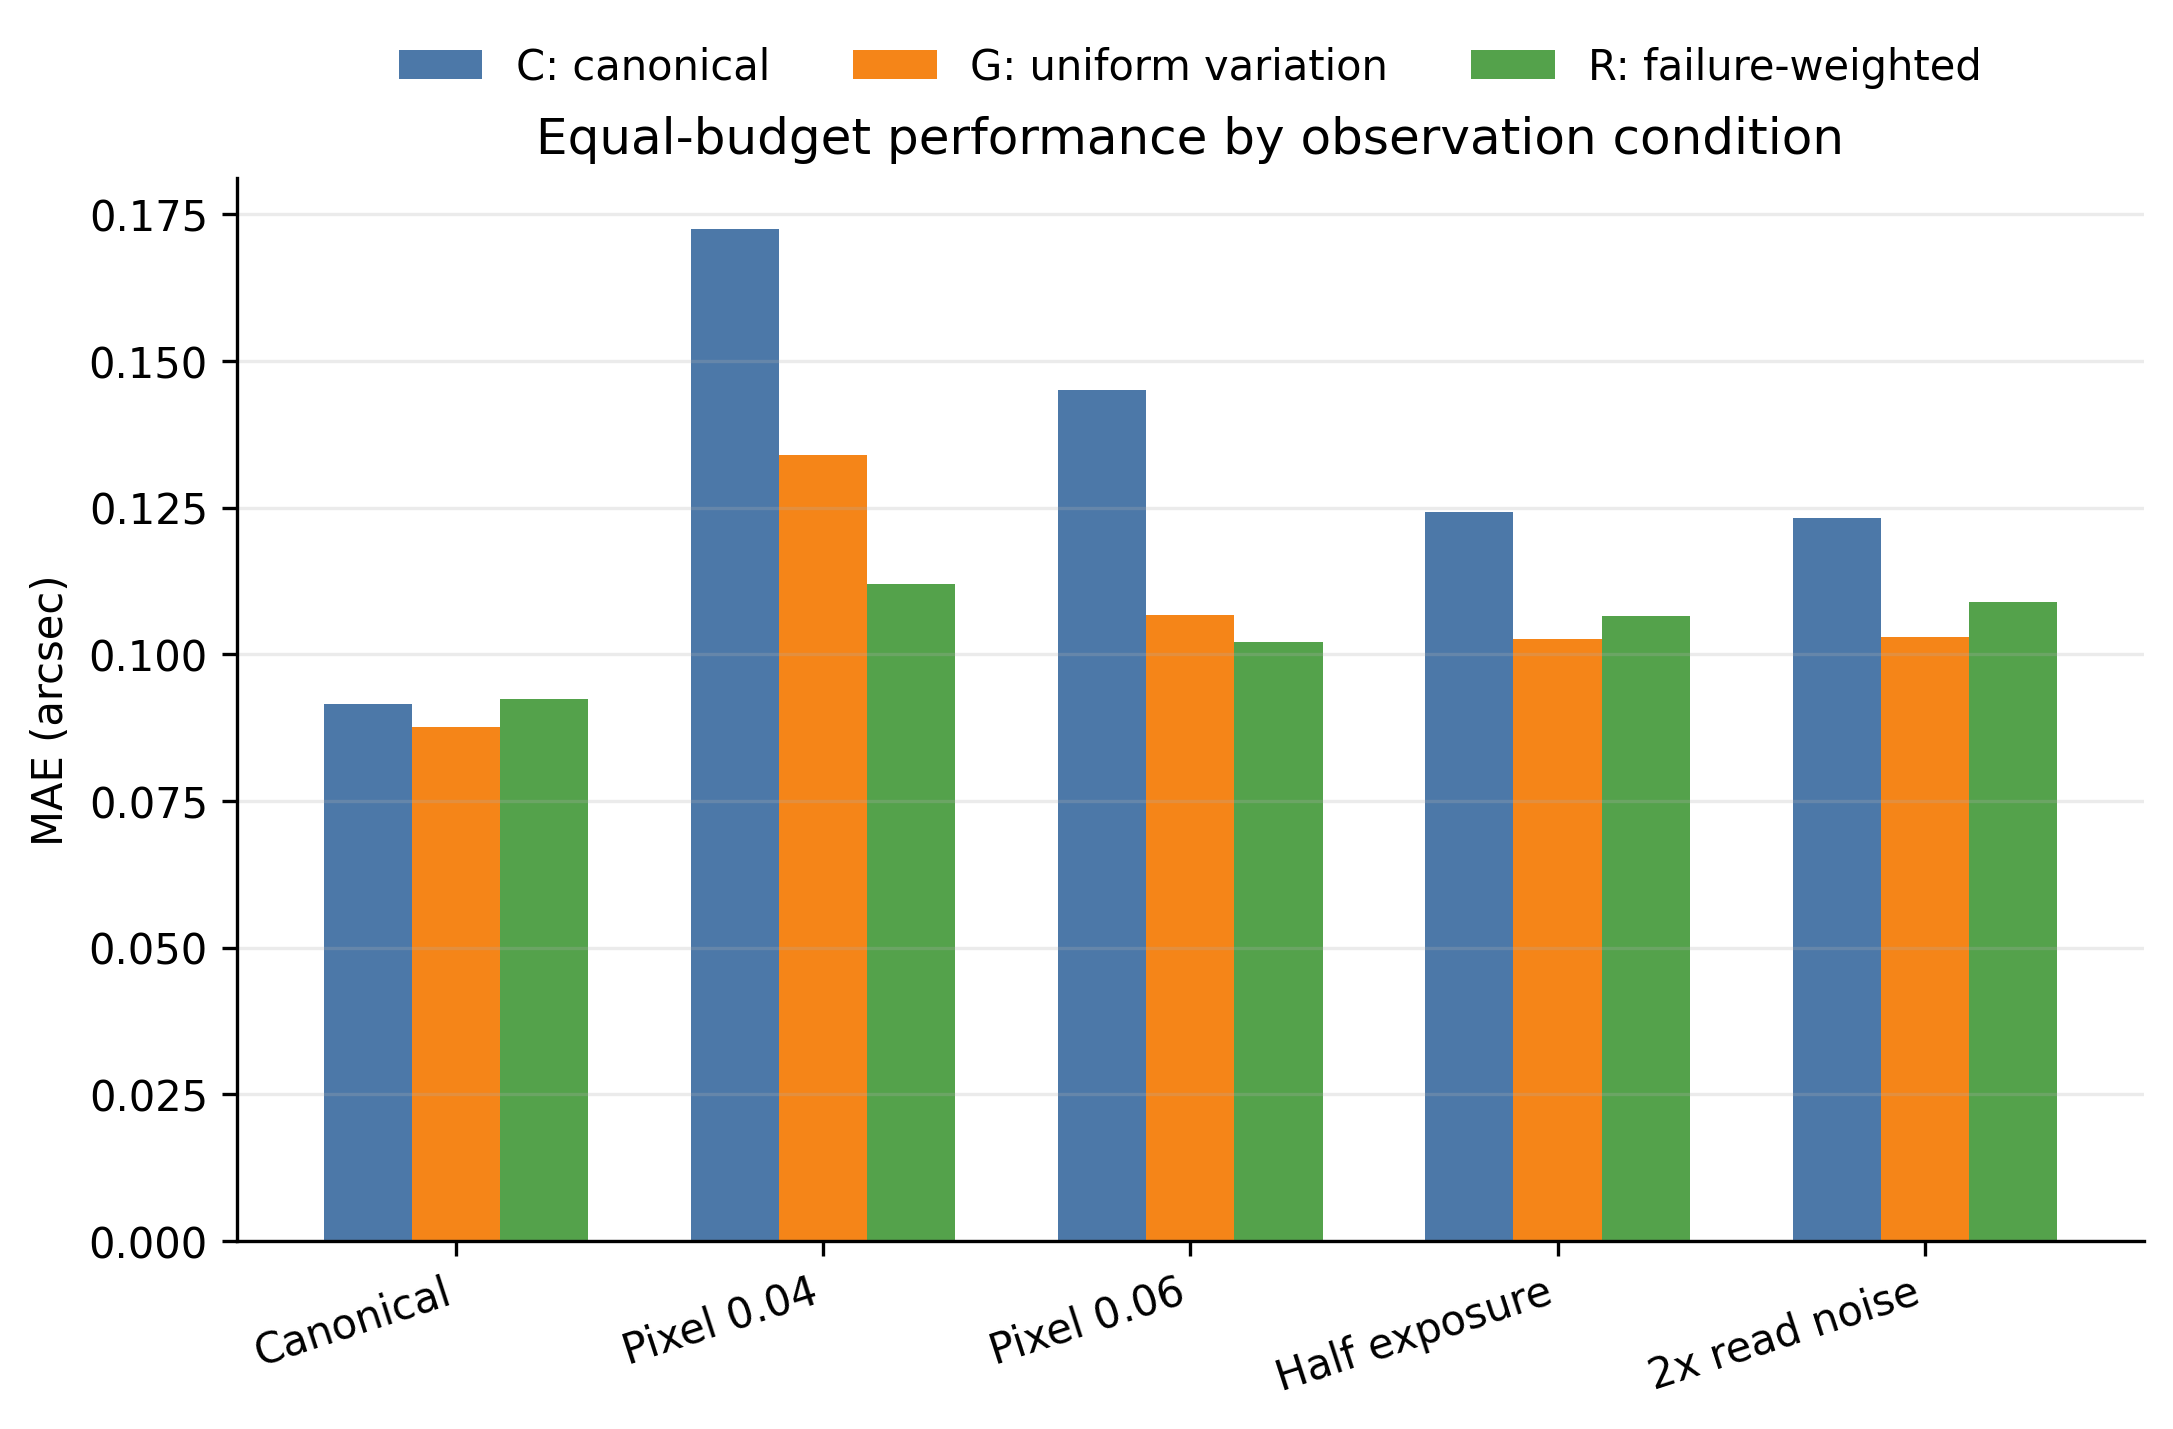
\includegraphics[width=\columnwidth]{figures/equal_budget_mae_by_condition.png}
\caption{MAE by image condition for the three training arms.}
\label{fig:mae}
\end{figure}

\begin{figure}[t]
\centering
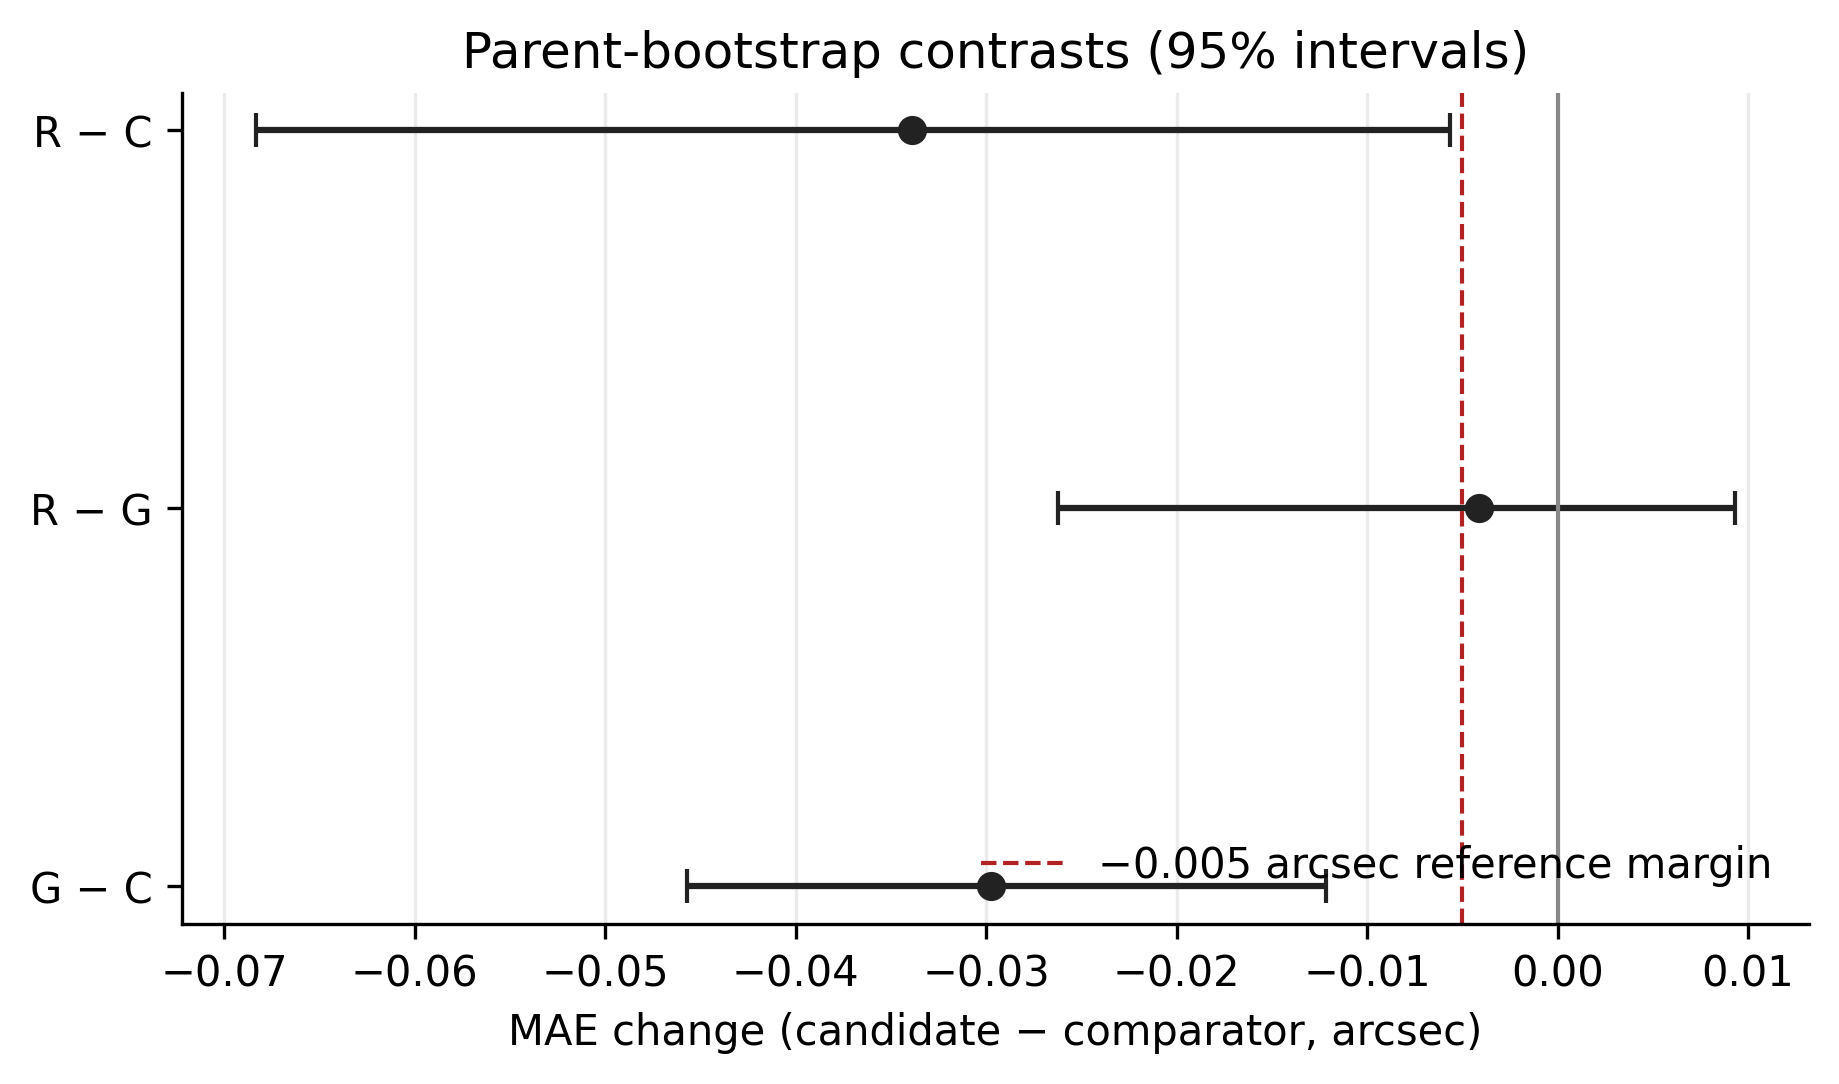
\includegraphics[width=\columnwidth]{figures/equal_budget_paired_contrasts.png}
\caption{Bootstrap intervals for paired differences. Negative values favor the
candidate arm.}
\label{fig:contrasts}
\end{figure}

R obtained a lower four-stress point estimate than G, but the R-minus-G
difference was -0.004122 arcsec with a 95\% interval of
[-0.026208,0.009341]. The data do not establish a reliable advantage for
difficult-condition sampling.

The earlier 27.4\% improvement came from a comparison with unequal update and
image-exposure budgets. We retain it as historical context, but the matched
budget result above is the primary comparison in this paper.

\subsection{Image-Generation Comparison}

All 1,350 paired image products and all 40,500 paired predictions were exactly
equal at the saved float32 precision. The Moffat conditions therefore test an
unseen PSF family shared by both implementations. They do not provide evidence
of transfer to an independent simulator.

\section{Limitations}

The study uses one synthetic parent distribution, one scalar target, and a
project-specific PSF, detector model, and preprocessing method. The Moffat PSF
conditions are engineered synthetic data, not calibrated telescope PSFs.

The two image-generation implementations share parts of the image-formation
and preprocessing pipeline. Their identical outputs are therefore a control
result, not a successful independent-simulator test. A future cross-simulator
study must produce a verified input difference before comparing model
performance.

The holdout is separate from the training parents, but older models were
previously evaluated on it. The present work is a new matched-budget refit on a
frozen holdout, not a never-before-opened dataset. No real-image
$\theta_E$ labels were used. We did not reproduce the Swierc or Agarwal methods
on this holdout, so we make no numerical superiority claim over those papers.

\section{Conclusion}

Under a matched training budget, uniform variation of image conditions reduced
four-stress Einstein-radius error on unseen synthetic parent systems. A policy
that sampled difficult conditions more often did not show a reliable
improvement over uniform sampling.

The result supports a controlled synthetic robustness conclusion. It does not
establish simulator-independent inference, real-data accuracy, or superiority
over published methods.

\section*{Reproducibility}

The submission supplement contains the aggregate result tables, figures, and a
reviewer-safe description of the training and evaluation protocol. The main
result uses fixed parent splits, paired seeds, sealed predictions, and
parent-level bootstrap intervals. No real-data score is included.

\bibliographystyle{aaai2027}
\bibliography{paper}

\end{document}
